\documentclass[12pt,twoside]{article}
\usepackage{amsmath, amssymb}
\usepackage{amsmath}
\usepackage[active]{srcltx}
\usepackage{amssymb}
\usepackage{amscd}
\usepackage{makeidx}
\usepackage{amsthm}
\usepackage{algorithm}
\usepackage{algpseudocode}
\usepackage{fancyhdr}
\usepackage{graphics}
%----------------------------------------------------------------------------------------------
\usepackage{amsmath, amssymb}
\usepackage{amsmath}
\usepackage[active]{srcltx}
\usepackage{amssymb}
\usepackage{amscd}
\usepackage{makeidx}
\usepackage[dvips]{graphicx}
\usepackage{longtable}
\usepackage{tabularx}
\usepackage[table,xcdraw]{xcolor}
\usepackage{color}
\usepackage[hidelinks]{hyperref}
\usepackage[backend=biber,style=apa]{biblatex}
\renewcommand{\tablename}{Tabla}
\renewcommand{\figurename}{Figura}
\renewcommand{\baselinestretch}{1}
\setcounter{page}{1}
\setlength{\textheight}{21.6cm}
\setlength{\textwidth}{14cm}
\setlength{\oddsidemargin}{1cm}
\setlength{\evensidemargin}{1cm}
\pagestyle{myheadings}
\thispagestyle{empty}
\markboth{\small{Pr\'actica 1. Luis Francisco Renteria Cedillo, Denzel Omar Vazquez Perez.}}{\small{.}}
\date{}
\begin{document}
\begin{figure}[h]
\vspace{-3cm} \hspace{-2cm} \setlength{\unitlength}{1mm}
\begin{picture}(15,25)(-10,0)

\includegraphics[width=16.5cm,height=3.5cm]{imagenes/titulo.png}
\end{picture}
\end{figure}
\vspace{0cm}
\centerline{\bf An\'alisis de Algoritmos, Sem: 2022-2, 3CV11, Pr\'actica 1, 2 de marzo de 2022}
\centerline{}
%\centerline{}

\begin{center}
\Large{\textsc{Pr\'actica 1: Determinaci\'on experimental de la complejidad temporal de un algoritmo}}
\end{center}
\centerline{}
\centerline{\bf {Luis Francisco Renteria Cedillo, Denzel Omar Vazquez Perez.}}
\centerline{}
\centerline{$lrenteriac1400@alumno.ipn.mx, dvazquezp1600@alumno.ipn.mx$}



\newtheorem{Theorem}{\quad Theorem}[section]

\newtheorem{Definition}[Theorem]{\quad Definition}

\newtheorem{Corollary}[Theorem]{\quad Corollary}

\newtheorem{Lemma}[Theorem]{\quad Lemma}

\newtheorem{Example}[Theorem]{\quad Example}

\bigskip

\textbf{Resumen:} En el presente documento se plantean dos problemas junto con su respectiva soluci\'on cuyo objetivo es determinar el orden de complejidad temporal de los algoritmos dados. Posteriormente se presentará una gr\'afica que muestre una función que acote los l\'imites de los pares ordenados que presentaron ambos algoritmos dadas unas condiciones iniciales.

{\bf Palabras Clave:} Complejidad temporal, Euclides, Fibonacci, C.

\section{Introducci\'on}
    Un algoritmo se puede definir como una serie de instrucciones que representan un modelo para solucionar ciertos tipos de problemas. Los algoritmos se utilizan en gran parte de las ciencias de la computación. Es por eso que el diseño de algoritmos requiere una amplia gama de conocimientos de programaci\'on y aplicar en múltiples casos la creatividad.
    
    Eficacia vs Eficiencia:
    un algoritmo es eficaz si puede encontrar una soluci\'on a un problema determinado, sin embargo, esta capacidad puede volverse muy compleja cuando se busca una soluci\'on \'optima. Es aqu\'i cuando entra la eficiencia que se define como la relaci\'on entre recursos utilizados de un sistema y los logros conseguidos con el mismo. Dicho de otra forma, un buen algoritmo es correcto, pero un gran algoritmo es correcto y adem\'as eficiente.
    
    Dado este enfoque, el an\'alisis de algoritmos toma un papel importante a la hora de desarrollar software, ya que, podemos calcular una aproximaci\'on del comportamiento de un algoritmo. Con esto podemos comparar diversos algoritmos y escoger el que mejor se adapte para lograr nuestro prop\'osito.


\section{Conceptos B\'asicos}
\subsection{Complejidad algor\'itmica}
    La complejidad algor\'itmica es una medida de cuánto tiempo tarda en completarse un algoritmo dada una entrada de tama\~no n, calculando el resultado dentro de un límite de tiempo finito y práctico incluso para valores grandes de n. Si bien la complejidad generalmente se expresa en términos de tiempo también se analiza en términos de espacio, lo que se traduce en los requisitos de memoria del algoritmo.
\subsubsection{Complejidad temporal}
    Se define como la eficiencia en tiempo siendo el numero de pasos ejecutados para resolver un problema con una entrada de tama\~no n, se denota por T(n).
\subsubsection{Complejidad espacial}
Al igual que la anterior, existe la eficiencia en espacio que hace referencia a la cantidad de recursos de memoria que utiliza el algoritmo para resolver un problema con una entrada de tama\~no n, se denotada por S(n).
\subsection{Notaci\'on $\Theta$}
La notación Theta ($\Theta$) es un modo de denotar lo que es el límite asintótico de la tasa de crecimiento del tiempo de la ejecución de un algoritmo considerando el límite superior e inferior. Básicamente define el comportamiento asintótico exacto, se puede describir en t\'erminos formales como:
$$\Theta(g(n)) = \{ f(n)~\arrowvert~\exists_{n}~C_{1},~C_{2}>0~\&~n_{0}>0~tal~que$$ $$0\leq~C_{1}g(n)~\leq~f(n)~\leq~C_{2}g(n)~\forall~n\geq~n_{0}\}$$
\subsection{Notaci\'on $\mathcal{O}$}
Dado un $f(n)$ que muestra la complejidad de un algoritmo en función de una entrada de tama\~no n , la expresión $f(n)$ $\in$ $\mathcal{O}(g(n))$ indicando que $f(n)$ no crece más de prisa que $g(n)$, donde esta \'ultima es denominada cota superior asintótica. $\mathcal{O}(g(n))$ es un conjunto que que se puede describir en t\'erminos formales como:
$$\mathcal{O}(g(n)) = \{ f(n)~\arrowvert~\exists_{n}~C_{1}>0~\&~n_{1}>0~tal~que$$$$0\leq~f(n)~\leq~C_{1}g(n)~\forall~n\geq~n_{1}\}$$
\subsection{Notaci\'on $\Omega$}
La notación $\Omega$ es lo inverso a $\mathcal{O}$, por lo que se puede definir como una función que sirve de cota inferior de otra función cuando el argumento tiende a infinito, en t\'erminos formales se puede describir como:
$$\Omega(g(n)) = \{ f(n)~\arrowvert~\exists_{n}~C_{1}>0~\&~n_{1}>0~tal~que$$$$0\leq~C_{1}g(n)~\leq~f(n)~\forall~n\geq~n_{1}\}$$
\subsection{Algoritmo para comparar dos arreglos}
Siendo un problema computacional que debe encontrar de un arreglo $A$ con n elementos enteros positivos,  un elemento $K$, donde si $K~\in$ al subarreglo $A[0, ... , ^n/_2-1]$ tanto a $A[^n/_2, ... , n-1]$, se devuelve el valor del elemento $K$.\\
El pseudo-c\'odigo para la implemetaci\'on de este es:\\[.75cm]
    \textit{\large Busqueda(A,n):}
    \begin{algorithmic}
        \For{i$\leftarrow$0 to $^n/_2 -1$}
            \State \For{i$\leftarrow ^n/_2$ to $n-1$}
                    \State \If{A[i]==A[j]}
                        \State {Mostrar A[i], i, j}
                        \EndIf
                \EndFor
        \EndFor
        \State{Mostrar “No se encontraron coincidencias”}
    \end{algorithmic}
\subsection{Algoritmo de Euclides}
Es un algoritmo eficiente para encontrar el \textit{mcd} (m\'aximo com\'un divisor) de dos n\'umeros enteros positivos m y n. Este algoritmo fue propuesto por el matem\'atico griego Euclides, en el libro \textit{"The Elements"}.\\
El pseudo-c\'odigo para la implemetaci\'on de este es:\\[.75cm]
    \textit{\large Euclides(m, n):}
    \begin{algorithmic}
        \While{ n $\neq$ 0}
            \State {r $\leftarrow$ m $\mathrm{mod}$ n}
            \State {m $\leftarrow$ n}
            \State {n $\leftarrow$ r}
        \EndWhile
        \State {return m}
    \end{algorithmic}
\section{Experimentaci\'on y Resultados}
    \subsection{Algoritmo para comparar dos arreglos}
    El primer algoritmo, genera un numero aleatorio par que determina el tamaño de un arreglo A, una vez hecho esto, se genera m\'ultiples n\'meros aleatorios que tienen un valor desde 0 hasta 3n, mismos que se utilizan para rellenar dicho arreglo A. 
    Se crea la funci\'on de b\'usqueda que tiene como argumentos el arreglo A y su longitud n. Posteriormente se codifica dos ciclos for anidados, el primero controla el \'indice del subarreglo de la primera mitad y el segundo ciclo controla el \'indice del subarreglo correspondiente a la segunda mitad del arreglo.
    Si la condici\'on de que el valor en el \'indice i es igual al valor en el \'indice j, la funci\'on se detiene y regresa tanto los \'indices como el valor repetido.
    
    Ejecutando el c\'odigo se obtiene un conjunto de pares ordenados, el eje de las abscisas representa la longitud n y el eje de las ordenadas el n\'umero de operaciones. Estos datos son guardados en un archivo csv.
    
    A continuación se observa la gr\'afica de n vs n\'umero de operaciones:
    
\begin{figure}[H]
    \centering
    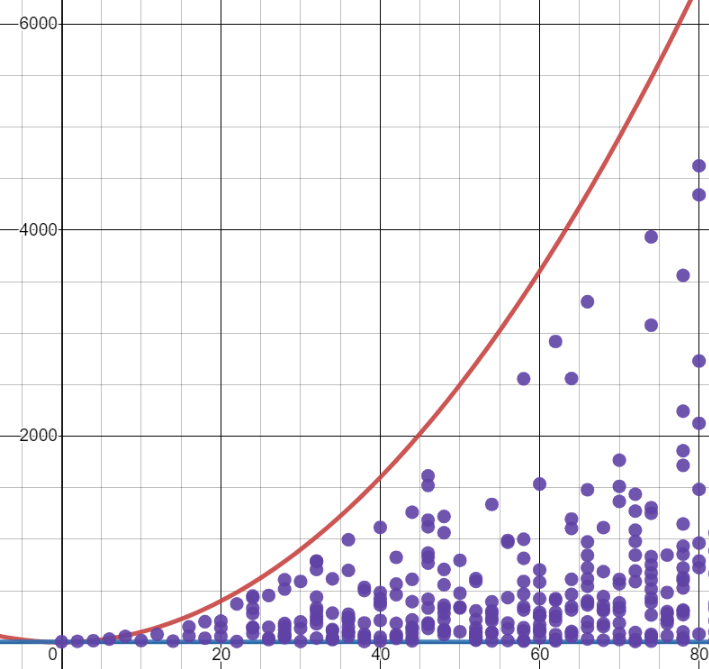
\includegraphics[height=6.5cm , width=7.5cm]{imagenes/grafica1a.png}
    \caption{Gr\'afica de n vs n\'umero de operaciones}
\end{figure}
Se observa en el plano cartesiano que el algoritmo de b\'usqueda tiene, en el peor caso, un comportamiento de una funci\'on cuadr\'atica. La cota superior g(n)= n$^{2}$ mientras que la cota inferior es la constante de 4, representando el mejor caso. Por lo tanto, el peor caso esta dado por T(n)=n$^{2}$ $\in O(n ^2)$ y el mejor caso por T(n)=4 $\in \Omega(1)$

A continuación se muestra la salida de ejecuci\'on  del c\'odigo, podemos apreciar los valores del arreglo y el valor repetido en sus posiciones i,j. Incluso podemos ver que la \'ultima ejecución no encontr\'o coincidencias.
\begin{figure}[H]
    \centering
    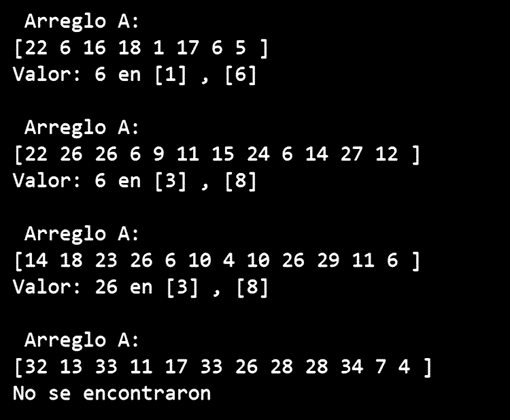
\includegraphics[height=6cm]{imagenes/salida1.png}
    \caption{Resultados de los casos prueba en el algoritmo de B\'usqueda.}
\end{figure}

    
    \subsection{Algoritmo de Euclides}
Posteriormente al ejecutar el programa con la funci\'on creada con el nombre \textit{"Euclides"}, se tiene que la asignación de valores de entrada m y n esta dada por la secuencia Fibonacci, por tanto se obtiene el n\'umero de operaciones, los resultados registrados se muestran en la Tabla 1.
    \begin{longtable}{|l|l|l|}
        \caption{Complejidad temporal del algoritmo de Euclides}\\
            \hline
                \textbf{m}&\textbf{n}&\textbf{T(n)}\\
            \hline
                {1}&{1}&{6}\\
            \hline
                {1}&{2}&{10}\\
            \hline
                {2}&{3}&{14}\\
            \hline
                {3}&{5}&{18}\\
            \hline
                {5}&{8}&{22}\\
            \hline
                {8}&{13}&{26}\\
            \hline
                {13}&{21}&{30}\\
            \hline
                {21}&{34}&{34}\\
            \hline
                {34}&{55}&{38}\\
            \hline
                {55}&{89}&{42}\\
            \hline
                {89}&{144}&{46}\\
            \hline
                {144}&{233}&{50}\\
            \hline
    \end{longtable}
Al considerar como peor caso los valores m y n de la Tabla 1, se procede a graficar los puntos sobre el plano cartesiano.
\begin{figure}[H]
    \centering
    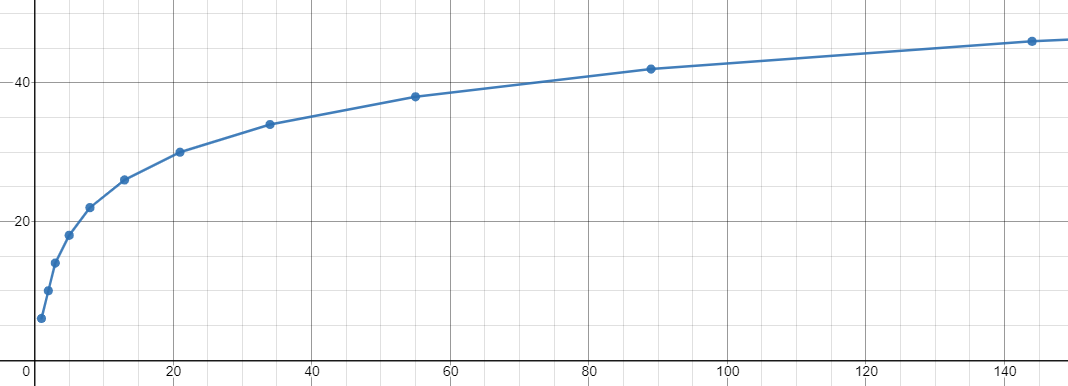
\includegraphics[height=5cm]{imagenes/grafica321.png}
    \caption{Resultados de los casos prueba en el algoritmo de Euclides.}
\end{figure}
A partir de la Figura 3 se observa que el comportamiento del el peor caso es logar\'itmico por tanto T(n) = K log(n),con el fin de acotar por arriba a la funci\'on original, se tiene que 20 log(n) es una cota superior, por lo que todo resultado experimental se encuentra acotado por abajo por T(n)=6 $\in \Omega(1)$  (mejor caso) y por arriba por T(n)=20 log(n) $\in O(\log{}n)$ como se ve en la Figura 4.
\begin{figure}[H]
    \centering
    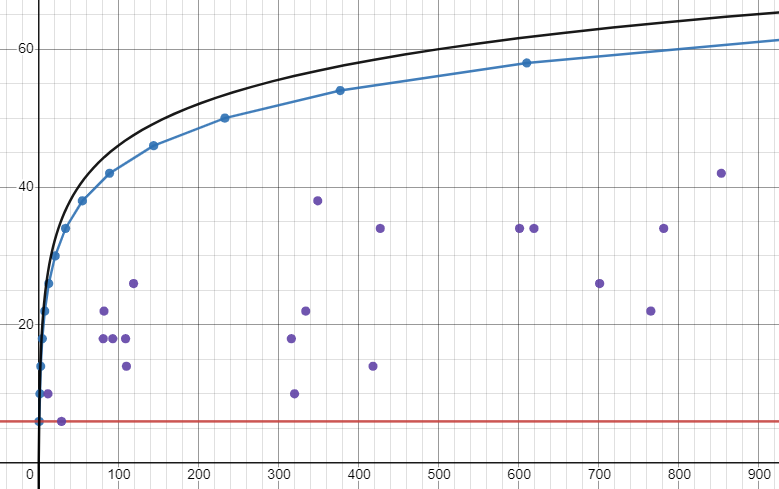
\includegraphics[height=7cm]{imagenes/grafica322.png}
    \caption{Gráfico del peor y mejor caso para el algoritmo de Euclides}
\end{figure}

\newpage 

\section{Conclusiones}
\textbf{\large Luis Francisco Renteria Cedillo}
\begin{figure}[H]
    \centering
    
\includegraphics[angle=0, scale=0.5]{imagenes/foto1.png}
\end{figure}

Un algoritmo debe analizarse para determinar la cantidad de recursos que utiliza en el sistema. Es importante mencionar que existen diversas formas de medir la eficiencia de un algoritmo, pero el arquitecto del sistema debe dar prioridad sobre una, como por ejemplo, complejidad temporal por encima de complejidad espacial.
En el análisis del algoritmo, fue vital comprender cuando una instrucción es ejecutada aunque no se vea explícitamente en el código. Como ejemplo tenemos que un ciclo for realiza una ejecución extra antes de salir del bucle, donde se verifica que una condición no se cumple, y por tanto, termina el ciclo.\\[1.2cm]
\textbf{\large Denzel Omar Vazquez Perez}
\begin{figure}[h]
    \centering
    
\includegraphics[angle=-90, scale= 0.05]{imagenes/foto2.jpg}
\end{figure}

El pensamiento y codificaci\'on de cada algoritmo influye directamente en la complejidad que tendr\'a este, siendo de ejemplo el primer problema de la b\'usqueda de un elemento similar en los sub-arreglos previamente creado, donde los dos puntos anteriormente dichos son los intermediarios para determinar que tan eficaz sera la soluci\'on del problema, en este caso se propuso mostrar el peor caso con complejidad $O(n ^2)$, sin embargo es importante mencionar que el haciendo uso de de la la estructura de datos hash es posible llegar a una complejidad $O(n)$. Para el segundo problema es sencilla su implementaci\'on haciendo el seguimiento del algoritmo proporcionado en la pr\'actica. 

\section{Bibliograf\'ia}

Brassard, G. (1997). \textit {Fundamentos de Algoritmia}. España: Ed. Prentice Hall.\\[0.4cm]
Cormen, E. A. (2022). \textit{Introduction To Algorithms}, 3Rd Ed. Phi.\\[0.4cm]
Devopedia. 2022. \textit{Algorithmic Complexity.} Version 8, February 19. Accessed 2022-02-19.\\[0.4cm] https://devopedia.org/algorithmic-complexity
Luna, Benjam\'in. \textit{Fundamentos para el an\'alisis de eficiencia algor\'itmica}. Escuela Superior de Computo, IPN. M\'exico. 28 de febrero de 2022.\\[0.4cm]
S\'anchez, P. J. I. (2006). \textit{Análisis y diseño de algoritmos: un enfoque teórico y práctico}. Servicio de Publicaciones y Divulgación Científica de la UMA.


\medskip

\end{document}